\documentclass[12pt]{article}
\usepackage{fullpage}
\usepackage{amsmath}
\usepackage{hyperref}
\usepackage{graphicx}
\usepackage{listings}
\usepackage{float}
\usepackage{alltt}
\usepackage{verbatim}

\floatstyle{plain}
\newfloat{snippet}{thb}{lop}
\floatname{snippet}{Snippet}

\newcommand{\mtt}[1]{\(#1\)}
\newcommand{\vrb}[1]{\verb=#1=}

\begin{document}
  \begin{center}
    \textbf{\large Out-of-Order SMIPS} \\
    6.375 Microarchitecture Design\\
    6 April 2011 \\
    
    \vspace{\baselineskip}
    
    \emph{Team}: David S. Greenberg and Bhaskar Mookerji
  \end{center}
  
  \begin{center}
      \textbf{Abstract}
  \end{center}
  \begin{quotation}
      For our 6.375 final project, we are implementing a out-of-order processor using Tomasulo's algorithm and 
      a reorder buffer. The following extends our high-level design to microarchitecture interfaces and 
      discusses, in detail, our pipeline functionality and current implementation status. Our current 
      implementation is available online at \url{https://github.com/mookerji/finalproject_6375}.
  \end{quotation}

\section{Tomasulo's Algorithm at a Glance}

Before getting into the details of Tomasulo's algorithm, let's try to understand it at a high level. An instruction set architecture (ISA) has a finite number of places in which
it can store variables. These places are called registers. Tomasulo's algorithm dynamically computes the dependencies between instructions so that instructions that
don't have data dependencies can run in parallel, while only the truly data-dependent instructions are run in sequence. This increases the throughput of the system by exploiting
instruction level parallelism (ILP). Tomasulo's algorithm can be seen as a dynamic hardware implementation of Static Single Assignment, a compiler technique that does
the same dependency calculations in software.

The core idea of Tomasulo's algorithm is that each ISA register has a corresponding physical register. Since instructions are dispatched in order but executed out of order,
we can associate the source operands of the instruction with the physical registers corresponding to the ISA registers used in the instruction. The destination register of
the instruction, however, is written to a new physical register, and the destination ISA register is updated to be linked to the new physical register. That way, every 
register is assigned once and only true dependencies affect execution.

Of course, hardware can't be allocated, and so Tomasulo's algorithm allocates the physical registers from a pool and releases registers back into the pool when there are
no more instructions using them as a source operand. The details of this are explained later.

\section{Problem\label{sec:problem}}
Although an elastic pipelined microprocessor is an improvement over an unpipelined processor, its performance suffers due to pipeline stalls.
There are three classes of stalls, two of which are eliminated by Tomasulo's algorithm.

The first class of stall is a Write-After-Read stall. This is where we see an instruction $A$ which reads from register $r_x$ followed by an instruction
$B$ which writes to the same register $r_x$. Normally, $B$'s execution is blocked by $A$ since they both need to access the same register. If $A$ has
several cycles of latency, then $B$ will be stalled until $A$ completes execution. Tomasulo's algorithm eliminates this false dependency by writing the
result of $B$ to a separate physical register, allowing $B$ to execute in parallel with $A$.

The second class of stall is a Write-After-Write stall. This is where we see an instruction $C$ which writes to a register $r_y$ followed by an instruction
$D$ which writes to the same register $r_y$. Normally, since both instructions need to write to the same ISA register, $D$ would be stalled until $C$ completed;
however, Tomasulo's algorithm allows them to execute in parallel since the instructions would each write to separate physical registers.

The third class of stall is a Read-After-Write stall, or a true data dependency. This is where instruction $E$ writes to register $r_z$, and then instruction $F$
reads from register $r_z$. Tomasulo's algorithm does nothing in this case, because since $F$ needs the result of $E$, it must be stalled until $E$ completes.

Let's look at an example snippet of code to understand an example situation in which Tomasulo's algorithm would help (Snippet~\ref{mulmovadd}).
In this simplified assembly language, the format of an instruction is $op$, $src_1$, $\left[src_2\right]$, $dst$; $src2$ is optional.

\begin{snippet}
\begin{verbatim}
mul r1, r2, r3
mov r3, r4
add r1, r2, r3
\end{verbatim}
\caption{Instruction sequence which would benefit from Tomasulo's algorithm}
\label{mulmovadd}
\end{snippet}

Let's assume that multiplies take 4 clock cycles, moves take 1 clock cycle, and adds take 2 clock cycles. Also, let's assume that fetching an instruction takes 1 clock cycle
and happens in parallel with execution. Then executing these instructions in sequence takes a total of 8 clock cycles--one cycle for the initial fetch, followed by each instruction
executing in sequence (Table~\ref{tab:simpleex1}). Since fetches are pipelined, we only see the fetch latency on the initial instruction. Now, if we are using Tomasulo's algorithm, we'll instead
see a total runtime of 6 clock cycles. To understand why, we can look at this table \ref{tab:tomasuloex1}.

\begin{table}
\begin{tabular}{l || c | c | c | c | c | c | c | c}
Cycle & 1 & 2 & 3 & 4 & 5 & 6  & 7 & 8 \\ \hline
Multiply & fetch & exec 1 & exec 2 & exec 3 & exec 4 & & \\
Move & & fetch & stall & stall & stall & exec & \\
Add & & & fetch & stall & stall & stall & exec 1 & exec 2 \\
\end {tabular}
\caption{Snippet \ref{mulmovadd} executed on a simply pipelined microprocessor}
\label{tab:simpleex1}
\end{table}

\begin{table}
\begin{tabular}{l || c | c | c | c | c | c}
Cycle & 1 & 2 & 3 & 4 & 5 & 6 \\ \hline
Multiply & fetch & exec 1 & exec 2 & exec 3 & exec 4 & \\
Move & & fetch & stall & stall & stall & exec \\
Add & & & fetch & exec 1 & exec 2 & \\
\end {tabular}
\caption{Snippet \ref{mulmovadd} executed on a microprocessor with Tomasulo's algorithm}
\label{tab:tomasuloex1}
\end{table}

\section{High-Level Design}

\begin{figure}[ht!]
    \centering
    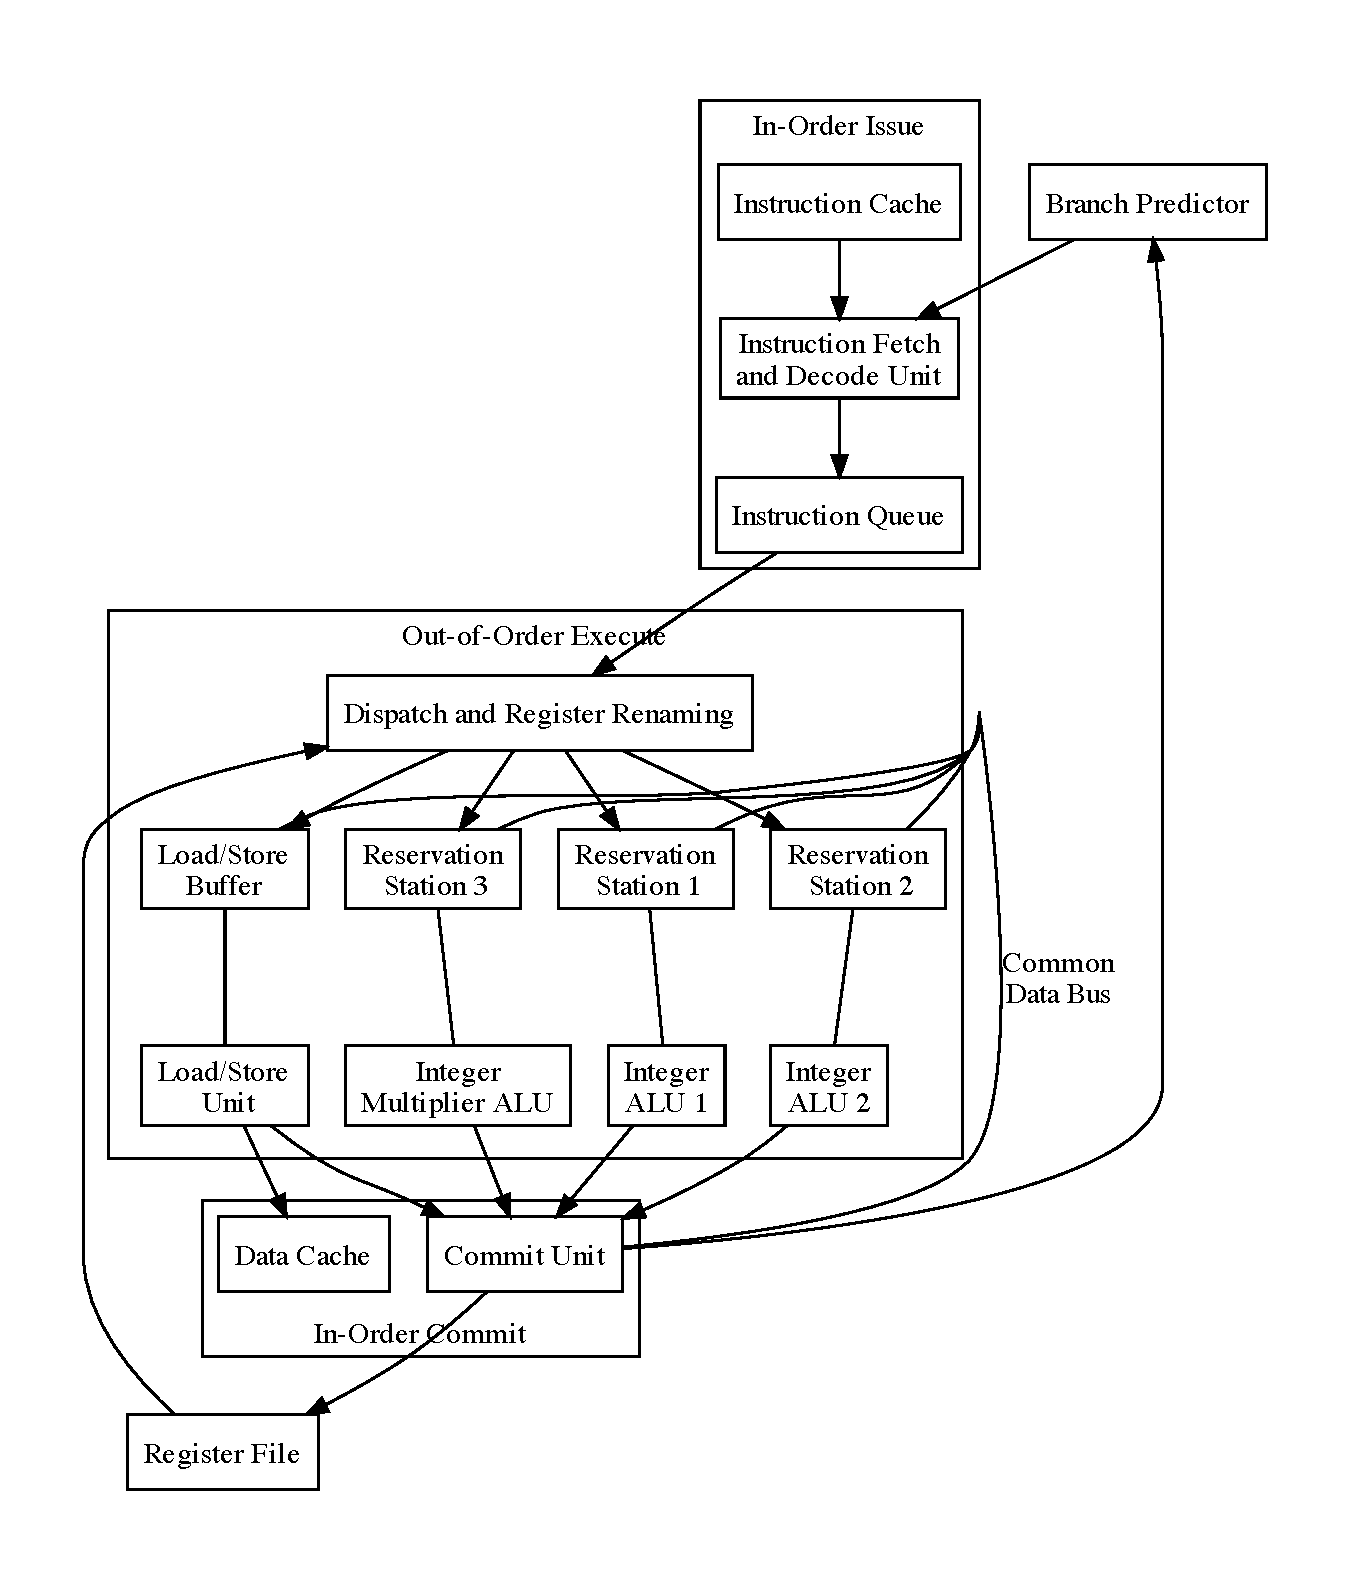
\includegraphics[width=\textwidth]{figures/design.pdf}
    \caption{System architecture using out-of-order execution and pipelined integer arthmetic. \label{fig:design}}
\end{figure}

\begin{figure}[h]
    \centering
    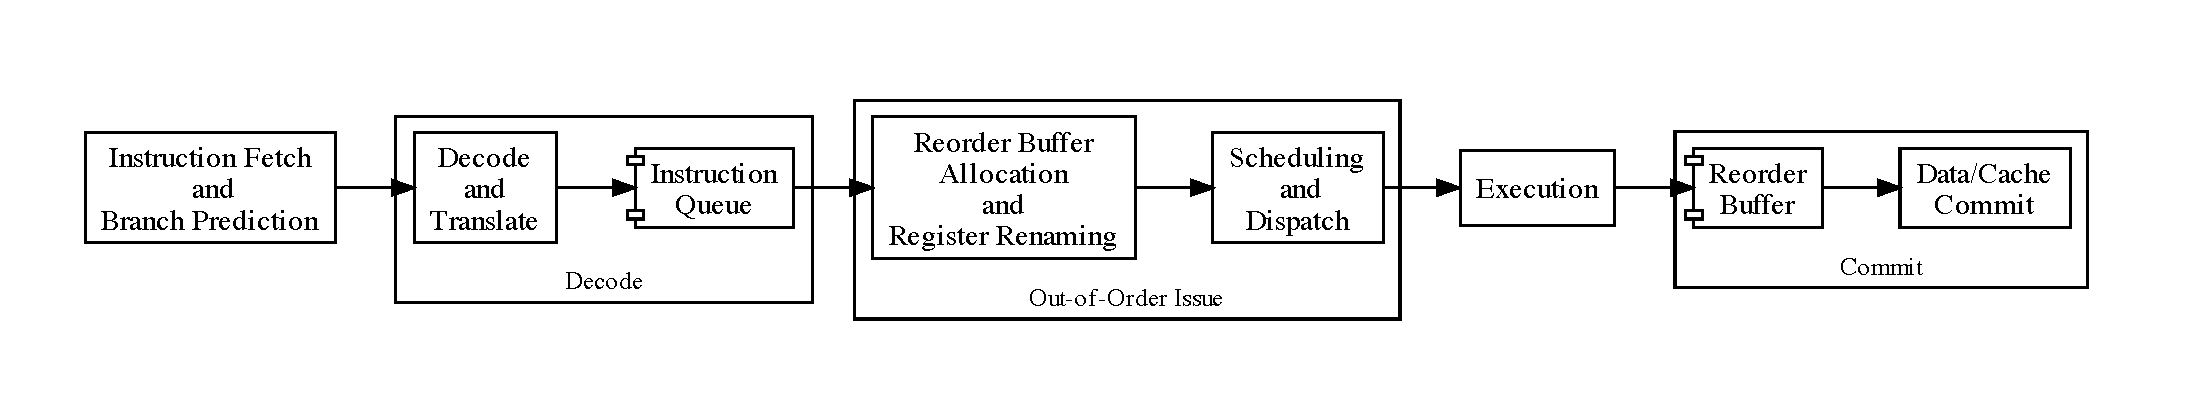
\includegraphics[width=1.1\textwidth]{figures/pipeline.pdf}
    \caption{Instruction pipeline. Pipeline stage is labeled in-box, unless superseded by an overbox. A component box indicates component (such as a FIFO) between stages. Not included in this diagram is the reservation stations and load/store buffer in the execution stage.\label{fig:pipeline}}
\end{figure}

The system design and instruction pipeline for our implementation is described
in Figure~\ref{fig:design} and~\ref{fig:pipeline}, respectively. 
The design extends our existing SMIPSv2 
implementation into three components: in-order instruction fetch and decoding, 
out-of-order execution units, and a commit unit. The instruction fetch and 
decode stage enqueues and dispatches instructions to reservation stations 
matching the appropriate execution unit, reordering as necessary to remove the 
pipelining hazards described in Section~\ref{sec:problem}. When the reservation 
station contains the appropriate operands for a given instruction, execution 
proceeds, and results are broadcast on a common data bus to waiting reservation 
stations and the branch prediction unit. The commit unit is implemented as a 
reorder buffer, and performs in-order commits to memory and the register file. 
Taken together with dispatch and register renaming, the reorder buffer and the 
reservation stations implement Tomasulo's algorithm. The details of this implementation 
are described in~\cite{99KMP} and~\cite{0023143}.

\section{Goals and Testing Strategy}

\subsection{Functional Correctness}

We will use the existing SMIPS implementation and toolchain to provide inputs, gather 
outputs, log rule executions as traces, and benchmark our implementation. Verifying the 
correctness of the Tomasulo's algorithm implementation will first require modular refinement
of fundamental components, such as the reorder buffer and reservation stations, before 
they are incorporated into our existing SMIPS implementation. To formally verify functional correctness,
we can examine traces for two different areas: data consistency invariants and instruction 
completion/termination/stalling conditions\footnote{This criteria for functional correctness in Tomasulo's
algorithm are described in greater detail in Chapter 6 of 
\emph{Design and Evaluation of a RISC Processor with a Tomasulo Scheduler} at~\url{http://www.kroening.com/diplom/diplom/}}.  

To further check for bugs, we will unit test with short programs that 
emphasize particular issues: sequences of dependent instructions, sequences of independent
arithmetic instructions, small loops, atypical branch sequences, and memory operations. 
Verifying the traces for these smaller test programs will simplify execution debugging 
for the existing benchmarks.

\subsection{FPGA Synthesis}
We've removed all CAM from the system, and so we believe that we should be able to 
synthesize modulo routing constraints.

\subsection{Performance}
Raw performance is not the goal of this project. With this architecture, we might not 
reach the IPCs of the three-stage pipeline architecture in Lab 4. To demonstrate the 
improvement of out-of-order execution in our processor, we will artificially introduce 
latency into our execution units using pipelined integer arithmetic routines. Theoretical 
performance and correctness are the primary concerns. Our design 
should enable future developers to use  a modularized Tomasulo's algorithm to hide the 
latencies of their additional instructions.
Unfortunately, there is way to show a strict benefit to the elastic pipelined SMIPS 
processor, since all ALU ops and multiplies  are single cycle on an FPGA anyway, and any 
worthwhile multicycle operation is a project in and of itself to implement.


\section{Microarchitecture Overview}

The following describes, in detail, newly implemented modules and extensions that facilitate out-of-order 
execution using the Lab 5 and 6 SMIPS processor. Section~\ref{sec:types} describes new types introduced
in \verb=TomasuloTypes.bsv=, Section~\ref{sec:stages} provides pseudocode describing rule execution for 
a five-stage elastic pipeline in \verb=Processor.bsv= and \verb=ALU.bsv=, and Section~\ref{sec:modules} summarizes 
the architectural modules that contain these types during the pipeline execution. Due to the ad-hoc 
organization of this document, we recommend you read Sections~\ref{sec:types},~\ref{sec:stages}, 
and~\ref{sec:modules} in-parallel (Figures and reorganization are coming). 

\subsection{New System Types\label{sec:types}}

Oh boy!

\begin{enumerate}
    \item \textbf{Reorder Buffer Tag and Reorder Buffer Entry}. At instruction issue, a reorder buffer tag 
    (\verb=ROBTag=) is generated by a token request at the reorder buffer. Keeping track of this value eliminates 
    the need for associative lookup by providing an index directly into the ROB. The ROB itself contains 
    the entries (\verb=ROBEntry=) with the intended register destination, a \verb=Maybe#{data}= for a
    result, and mispredict and epoch fields for handling branch prediction. 
    \begin{alltt}
        typedef Bit#(4) ROBTag;
        
        typedef struct {
            Maybe#(Data) data;
            Maybe#(Tuple2(Addr,Addr)) mispredict;
            Rindx dest;
            Epoch epoch;
        } ROBEntry deriving (Bits, Eq);
    \end{alltt}
    
    \item \textbf{Rename Entry}. The rename entries are contained in the rename register file, which extend 
    the register file by indicating if the register file contents are valid, and if not, where the data 
    might be found through the reorder buffer.
    \begin{alltt}
        typedef union tagged {
            void Valid;
            ROBTag Tag;
        } RenameEntry deriving (Bits, Eq);
    \end{alltt}
    
    \item \textbf{Reservation Station Entry}. Entries for the reservation station (\verb=RSEntry=) store 
    the operands, the ROB tag of the instruction in the reservation station, and an instruction tag. The 
    instruction tag is used for dispatching during issue and execution, and may also be extended by a 
    immediate field if two other operands already exist. An \verb=Operand= is either a data immediate
    or a tag for the ROB instruction that produces the desired value. An \verb=Op_type= is used later
    for dispatching classes of instructions. 
    \begin{alltt}
        typedef union tagged {
            ROBTag Tag;
            Data Imm;
        } Operand deriving (Bits, Eq);
        
        typedef struct {
            InstrExt op;
            ROBTag tag;
            Operand op1;
            Operand op2;
        } RSEntry deriving (Bits, Eq);
        
        typedef enum {ALU_OP, MEM_OP, JB_OP} Op_type deriving(Eq);    
        
        typedef union tagged {
            struct {} LW;
            ...
            struct { Simm offset;  } BEQ;
            ...
        } InstrExt deriving (Bits, Eq);
    \end{alltt}
    \item \textbf{Common Data Bus Packet}. The CDB's bypasses a packet to reservation station entries, containing
    a data immediate, its appropriate operand tag, and an epoch for branch prediction.
    \begin{alltt}
        typedef struct {
            Maybe#(Data) data;
            ROBTag tag;
            Epoch epoch;
        } CDBPacket deriving (Bits, Eq);
    \end{alltt}
    \item \textbf{ALU Request and Response}. The \verb=ALUReq= and \verb=ALUResp= are passed to the ALU module.
    The \verb=ALUReq= uses a \verb=InstrExt= field to dispatch operations and bypasses the ROB tag through
    to the completion and writeback pipeline stages. Arithmetic operations are performed on \verb=op1= and 
    \verb=op2= to yield \verb=ans=. 
    \begin{alltt}
        typedef struct {
            InstrExt  op;
            Data      op1;
            Data      op2;
            ROBTag    tag;
        } ALUReq deriving (Eq, Bits);

        typedef struct {
            Data   ans;
            ROBTag tag;
        } ALUResp deriving (Eq, Bits);
    \end{alltt}
\end{enumerate}

\subsection{Pipeline Stage Behavior\label{sec:stages}}
The rules in \verb=Processor.bsv= implement an elastic pipeline intermediated by the container modules
described in Section~\ref{sec:modules}. This section will eventually be updated to include branch prediction
handling and stalling logic, and might accidentally omit memory operations. Some pseudocode details are lifted from~\cite{99KMP}.
\begin{enumerate}
    \item \textbf{Instruction Fetch}. During instruction fetch, the instruction is fetched and enqueued. This
    is implemented by the \verb=fetch= rule.
        
    \item \textbf{Instruction Decode and Issue}. The instruction is interpreted and dispatched to the appropriate
    reservation station. During the decode stage, the instruction is piecewise parsed into an instruction 
    tag, a possible instruction tag extensions, and its operands (either register sources or immediates). The 
    decode stage's primary job is to resolve the operand sources and values of a given instruction $I_i$. 
       \begin{alltt}
           if (\mtt{\exists} free RS for \mtt{I\sb{i}} and !ROB.full):
               RS.op =  \mtt{I\sb{i}}
               RS.tag = ROB.tail
               
               \mtt{\forall} operands \mtt{x} of \mtt{I\sb{i}}:
                   if (\mtt{R\sb{x.A}} is Valid):
                       RS.op\mtt{\sb{x}} = Valid \mtt{R\sb{x.A}}.data
                   else if (CDB.tag == \mtt{R\sb{x.A}}.tag):
                       RS.op\mtt{\sb{x}} = Valid CDB.data
                   else if (ROB[\mtt{R\sb{x.A}}.tag] is Valid):
                       RS.op\mtt{\sb{x}} = Valid ROB[\mtt{R\sb{x.A}}.tag].data
                   else
                       RS.op\mtt{\sb{x}} = Invalid with \mtt{R\sb{x.A}}.tag
                       
               if (\mtt{I\sb{i}} has desination register \mtt{y.A})
                   \mtt{R\sb{x.A}}.tag = ROB.tail
                   ROB[ROB.tail].dest = \mtt{y.A}
               else
                   ROB[ROB.tail].dest = 0
       \end{alltt}
       If the reservation station (RS) and reorder buffer (ROB) are available, a reservation station entry is 
       initiated, grabbing a ROB token. Here, the register address of operand $x$ is denoted by $x.A$. The decode 
       stage instantiates the RS entry by checking in three places: the register file, the common data bus, or the
       reorder buffer. If Invalid, the instruction tag is stored in the reservation station. Simultaneously, the 
       reorder buffer is updated with the issued instruction. This is implemented by the \verb=decode_issue= rule.
    \item \textbf{Dispatch}. During dispatch, the operands and instruction tag are passed for execution. 
        \begin{alltt}
            \mtt{\forall} operands x
                if (RS.op\mtt{\sb{x}} tagged Invalid with .tag and tag == CDB.tag)
                    RS.op\mtt{\sb{x}} = Valid CDB.data
        \end{alltt}
        The instructions currently reside in the reservation station, which is constantly snooping the 
        CDB to update it's operands. Once all operands are valid and the functional unit is ready to accept
        a new instruction, the functional unit is initialized. 
        \begin{alltt}
            if (\mtt{\exists} free RS with Valid RS.op\mtt{\sb{x}} \mtt{\forall}
                operands x and !FU.stall):
                
                FU.op = RS.op
                FU.tag = RS.tag
                FU.op\mtt{\sb{x}} = RS.op\mtt{\sb{x}}
        \end{alltt}
        The snooping is an implicit guard implemented by the reservation station entry module. The rest is 
        implemented by the \verb=dispatch_alu= and \verb=dispatch_mem= rules
        
    \item \textbf{Execute}. The arithmetic operation or memory operations are performed. This is
    described in greater detail in the ALU module details, although the dispatch and complete rules 
    interface with \verb=aluReqQ= and \verb=aluRespQ= FIFOS, which have direct connections to the ALU 
    module.
        
    \item \textbf{Completion}. The result of the execution is bypassed and updated into the ROB. The reservation
    station requests the CDB, the result and the tag are placed on the CDB, and the matching ROB entry 
    is tagged valid with the result. 
        \begin{alltt}
            if (FU has result and got CDB-ack):
                CDB.data = FU.result
                CDB.tag = FU.tag
                ROB[CDB.tag] = Valid CDB.data
        \end{alltt}
        This is implemented by the \verb=alu_compl= rule.
    \item \textbf{Graduate}. The ROB writes back the execution result to the register file. 
        \begin{alltt}
            if (!ROB.full and ROB[ROB.head] is Valid):
                \mtt{x} = ROB[ROB.head].dest
                R\mtt{\sb{x}}.data = ROB[ROB.head].data
                if (ROB.head == R\mtt{\sb{x}}.tag):
                    R\mtt{\sb{x}} = Valid
            
        \end{alltt}
        This is implemented by the \verb=graduate= rule.
\end{enumerate}

\subsection{Architectural Interfaces\label{sec:modules}}

The following describes the support architectural modules implemented in our design.

\begin{enumerate}

    \item \textbf{Reservation Stations}. The reservation stations enqueue the instructions, their operands, and 
    any appropriate tags, as an \verb=RSEntry=, until a functional unit is available. As soon as all the operands
    are available, they are dispatched to the actual functional unit. The reservation station module keeps track
    of when its operands are ready for evaluation. The \verb=put= method enqueues an \verb=RSEntry=. 
    \begin{alltt}
        interface ReservationStation;
          method ActionValue#(RSEntry) getReadyEntry();
          method Action put(RSEntry entry);
        endinterface
    \end{alltt}
    
    \item \textbf{Common Data Bus}. Execution units place their results, packed as \verb=CDBPacket=s, on 
    the common data bus (CDB) module. Currently, this action can only be done once in a single clock cycle.
    Units reading from the CDB are called listeners. The reservation station snoop the CDB for missing operand 
    immediates. All listeners must check the bus every cycle and must acknowledge before accepting a new value.
    The CDB also has a state method \verb=hasData= for enforcing pipeline guards during CDB snooping. 
    \begin{alltt}
        interface CommonDataBus#(type t, numeric type nlisteners);
          method Action put(t entry);
          method ActionValue#(t) get(Bit#(TLog#(nlisteners)) id);
          method Bool hasData();
          method Action dumpState();
        endinterface
    \end{alltt}
    
    \item \textbf{ALU}. The ALU module accepts an \verb=ALUReq= type request and responds with a \verb=ALUResp= 
    type response using a \verb=proc_server= \verb=Server#(ALUReq, ALUResp)= subinterface. This module is only 
    used when two operands are available and dispatched from the ALU's reservation station. 
    \begin{alltt}
        interface ALU;
            interface Server#(ALUReq, ALUResp) proc_server;
        endinterface
    \end{alltt}
    
    \item \textbf{Reorder Buffer}. The ROB module is just great: it ensures that completed instructions are 
    retired in program-order. It is implemented as a circular FIFO queue with head and tail pointers. Newly 
    issued instructions are put into the ROB entry indexed by the tail pointer, whose value is also used 
    to tag the result. By bypassing these tags through the pipeline stages, we use an ROB without the synthesis
    overhead of associative lookup. Updating of the head and tail pointers is handled internally, as well as the 
    retiring of ROB entries upon register writeback, with the \verb=getLast= and \verb=complete= methods. 
    The \verb=isEmpty= and \verb=isFull= methods indicate the state of the ROB. The \verb=reserve=, 
    \verb=update=, \verb=get= methods return a tag, update a tagged entry, and retrieve a tagged entry,
    respectively. The ROB module is also used in purging instructions of the wrong epoch and issuing a 
    mispredict if a branch has been mispredicted.
    
    \begin{alltt}
        interface ROB#(numeric type robsize);
          method ActionValue#(Bit#(TLog#(robsize))) reserve(ROBEntry robEntry);
          method Action update(Bit#(TLog#(robsize)) tag, ROBEntry robEntry);
          method Maybe#(ROBEntry) get(Bit#(TLog#(robsize)) tag);
          method ROBEntry getLast();
          method Action complete();
          method Bool isEmpty();
          method Bool isFull();
        endinterface
    \end{alltt}
    \item \textbf{Branch Predictor (BTB).} The branch predictor unit is implemented as branch target buffer. It
    stores the current epoch, returns a prediction given it's current state, confirms a prediction, and 
    alters state based on misprediction. 
    \begin{alltt}
        interface BranchPredictor#(numeric type btbsize);
        	method ActionValue#(Addr) predict();
        	method Addr confirmPredict(Addr currentPc);
        	method Epoch currentEpoch();
        	method Action mispredict(Addr srcPc, Addr dstPc);
        endinterface
    \end{alltt}

\end{enumerate}

    \section{Implementation Status and Testing Plans}

    We have implemented every component of the processor. We have begun to debug the system. Currently, we execute around 40 instructions, including several branches and loops before running into issues. We can pass around 15\% of the asm testbench.

    \section{Planned Design Exploration}
    
    Our first goal is to obtain functional out-of-order execution with speculation, and then improve IPC performance by optimizing rule/pipeline concurrency and FIFO choices (as in Lab 6). We will explore architectural parametrization and design choices on the IPC and timing critical path:    
    \begin{enumerate}
        \item Reorder buffer dimension
        \item Branch prediction strategies (BTB and 2-Bit)
        \item Register file bypassing and FIFO usage
        \item Multiple ALU instruction issue
        \item Artificial arithmetic and memory latency
    \end{enumerate}
    
    \bibliography{citations}
    \bibliographystyle{alpha}
    

 \end{document}

\begin{comment}
    \item \textbf{Issue and Dispatch Units.} 
    \begin{itemize}
        \item[] Inputs: Instruction FIFO
        \item[] Outputs: Reservation Station Entry FIFO to the various execute units' reservation stations.
        \item[] Uses: Requests ROB token and places ROB entry, updates register map with the ROB token.
        \item[] Rules: If ROB token available and instruction ready, unpack instruction, fill in the known operands, 
        dispatch to a reservation station. If store instruction, wait for ROB to empty and issue.
    \end{itemize}
\end{comment}
